% ============================================================
% CHAPTER 10: IMPLEMENTATION
% MCDA 5585 / 5586 Major Project Report
% Bhavik Kantilal Bhagat | A00494758 | Saint Mary's University
% ============================================================

\chapter{Implementation}
\label{chap:implementation}

\FloatBarrier

\section{Platform Overview: Four-Layer Architecture}
\label{sec:platform_overview}


I designed and built three deliverables during my co-op placement that together form a coherent four-layer observability stack. Figure~\ref{fig:platform_overview} shows how I structured the layers and how they relate to the underlying IA platform infrastructure.

\begin{figure}[htbp]
\centering
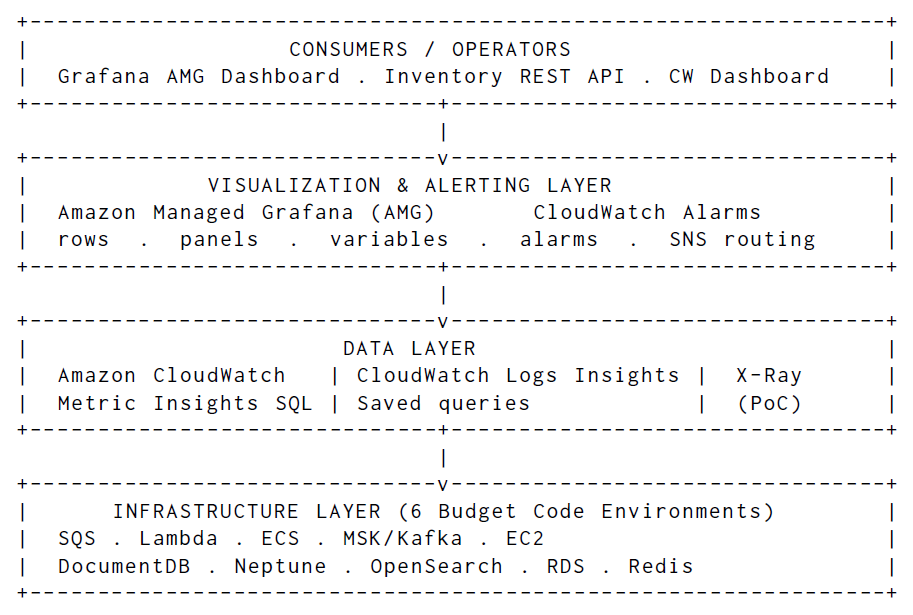
\includegraphics[width=0.95\textwidth]{figures/fig-ia-sre-observability-platform.png}
\caption[IA-SRE Observability Platform --- High-Level Architecture]{IA-SRE Observability Platform --- High-Level Architecture (four layers)}
\label{fig:platform_overview}
\end{figure}

Figure~\ref{fig:amg_system_arch} shows the full system architecture of the
Grafana AMG observability platform I built, detailing how each monitored AWS service
feeds CloudWatch, how the Lambda provisioner I wrote reads alarm templates from S3,
and how the SNS routing I configured delivers email notifications.

\begin{figure}[htbp]
\centering
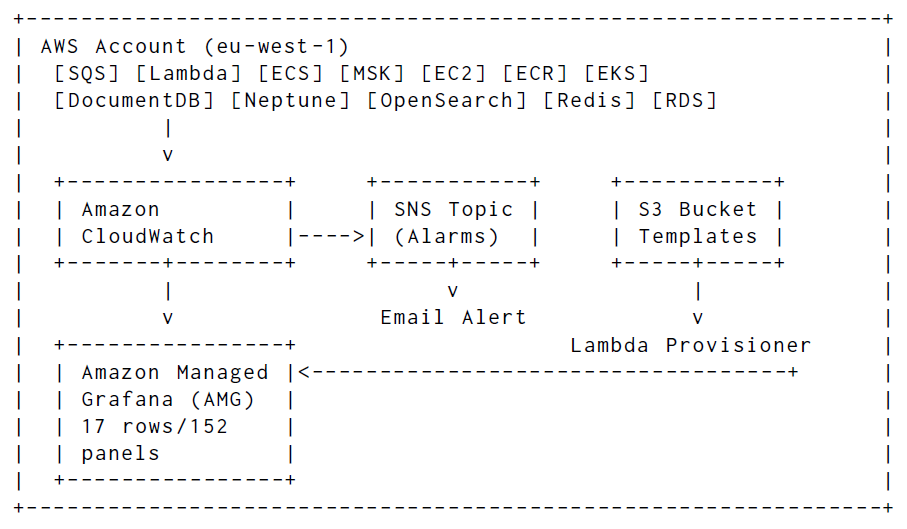
\includegraphics[width=0.95\textwidth]{figures/fig-amg-observability-platform.png}
\caption{AMG Observability Platform --- System Architecture}
\label{fig:amg_system_arch}
\end{figure}

The \textbf{infrastructure layer} is the monitored subject I targeted: six budget
platforms housing Lambda functions, ECS clusters, EC2
instances, and the full spectrum of AWS database and messaging services
used by the Meridian and CitcoWorks platforms.

The \textbf{data layer} ingests, stores, and queries observability signals
from the infrastructure layer. I chose Amazon CloudWatch as the sole data source ---
a deliberate architectural decision (see Section~\ref{sec:decision_cloudwatch_only})
that eliminates the operational overhead of a self-managed Prometheus stack.
I used CloudWatch Metric Insights SQL to provide per-resource aggregation, enabling
multi-service panels without requiring one panel per resource.

The \textbf{visualization and alerting layer} splits between two components I built.
I used Amazon Managed Grafana (AMG) to render the multi-row dashboard for human operators,
and I configured CloudWatch Alarms with SNS routing to fire notifications when metrics breach
their SLO-aligned thresholds.

The \textbf{consumers layer} includes three groups: operators who use the
Grafana dashboard I built during incident response, the IA Resources Inventory REST
API I developed that exposes the AWS service fleet programmatically, and the SRE team's
email distribution list that receives SNS alarm notifications I configured. This layered architecture ensures separation of concerns: the data layer handles metric collection and storage, the visualization layer transforms raw metrics into actionable insights, and the consumer layer delivers those insights to the appropriate stakeholders through purpose-built interfaces.


\FloatBarrier

\section{Work Stream 1: CloudWatch Dashboard Platform}
\label{sec:cw_dashboard_platform}


\subsection{Initial Lambda Dashboard}

My earliest monitoring work, completed in April~2026, produced a native
Amazon CloudWatch dashboard covering the \texttt{rpacfs1} and
\texttt{ia-bpo} Lambda function fleets --- 51 functions total. The dashboard
displayed per-function panels for invocation counts, error rates, duration
averages, and throttle events. I also created a Confluence inventory page
mapping each function.

The architectural pattern for this early work was straightforward:
CloudWatch native widgets queried the \texttt{AWS/Lambda} namespace using
\texttt{SEARCH()} expressions to enumerate all functions matching a
\texttt{FunctionName} prefix. This approach worked adequately for small,
homogeneous fleets but surfaced two structural limitations that drove
the later Metric Insights SQL migration: the \textbf{SEARCH() visibility
gap} (idle functions disappear from panels) and \textbf{no cross-environment
aggregation} (a single expression cannot span multiple tag dimensions
simultaneously).

Figure~\ref{fig:cloudwatch_dashboard} shows a live screenshot of the
CloudWatch Lambda dashboard displaying invocation and error metrics.

\begin{figure}[htbp]
\centering
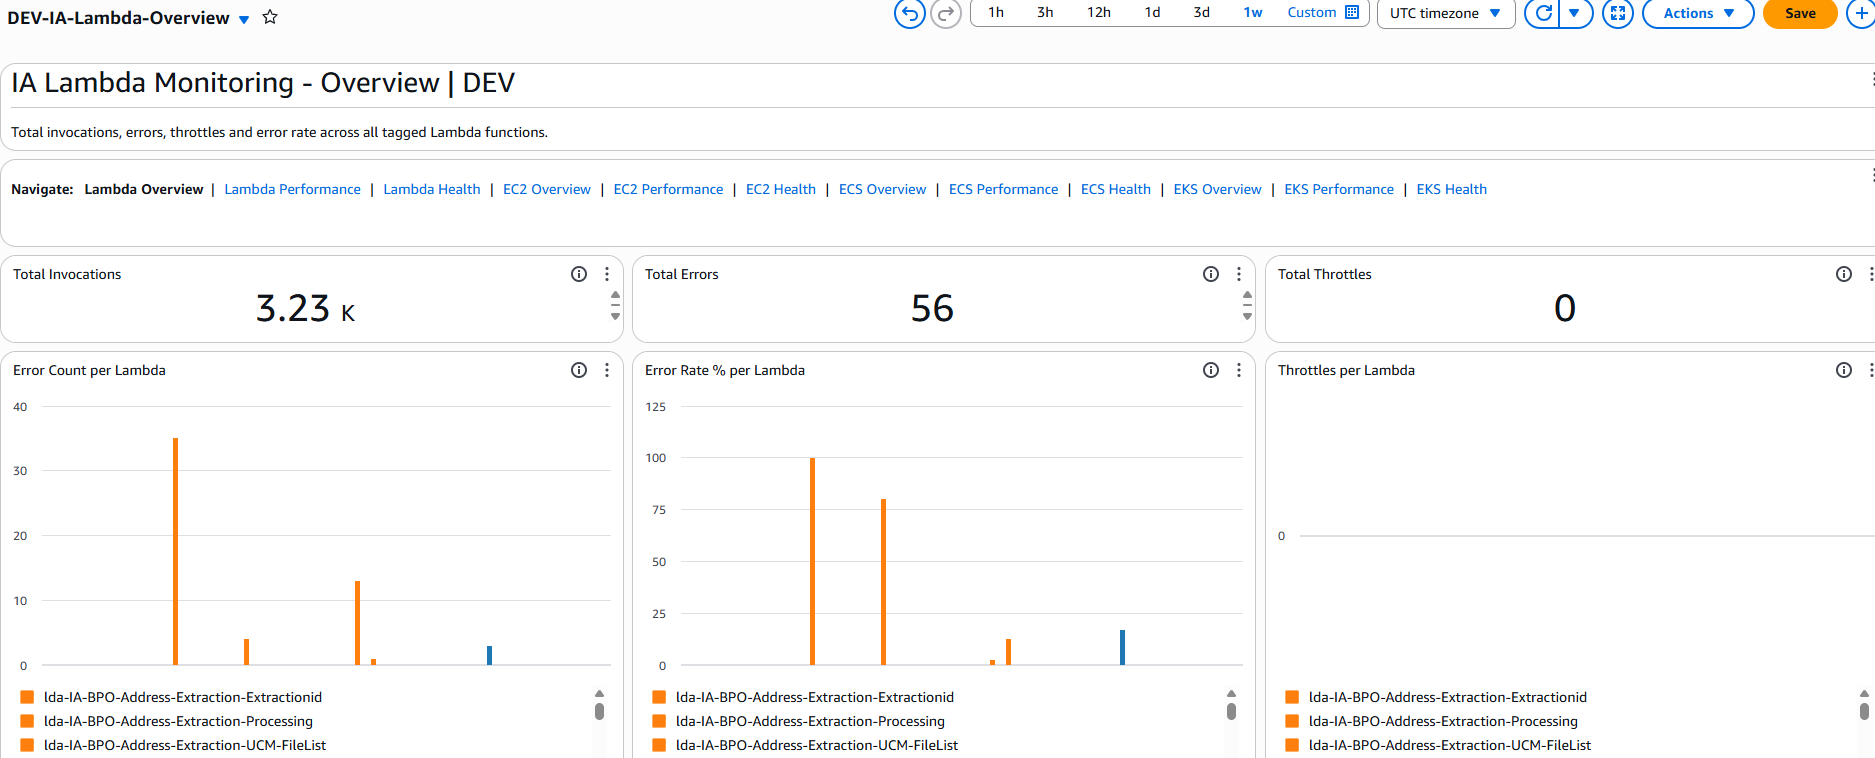
\includegraphics[width=0.95\textwidth]{figures/fig-cloudwatch-lambda-dashboard.png}
\caption[CloudWatch Lambda Dashboard --- Live Screenshot]{CloudWatch Lambda Dashboard --- Live Screenshot (ia-resources-monitoring)}
\label{fig:cloudwatch_dashboard}
\end{figure}

\subsection{Extended Dashboard and Architecture Analysis}

I extended the initial dashboard with additional tag dimensions
covering \texttt{automationhub}, \texttt{bpm}, \texttt{citcoworks}, 
and \texttt{meridian} budget\_codes, and introduced CloudWatch Logs Insights 
widgets for error log surfacing. 
Rather than relying solely on \texttt{Errors} metrics from
the \texttt{AWS/Lambda} namespace, the Logs Insights widgets queried the
\texttt{/aws/lambda/} log group prefix directly, enabling pattern-matched
error extraction regardless of whether Lambda had published a
corresponding metric.

A significant architectural investigation within this task evaluated the
feasibility of a fully centralized log aggregation approach using
CloudWatch metric subscription filters. My analysis quantified the
infrastructure cost of this design: routing log events from all IA Lambda
functions into a centralized processing layer would require \textbf{106
metric subscription filters}---one per function per metric
dimension---across the six platforms. While technically
feasible from a CloudWatch service quota perspective, this approach was
ultimately blocked by an IAM permission boundary constraint:
the \texttt{logs:PutSubscriptionFilter} action was not granted within the
IA team's scoped permission set, preventing programmatic creation of
subscription filters at the scale required.

This investigation also evaluated five distinct approaches to out-of-memory
(OOM) detection for Lambda functions: (1) parsing \texttt{REPORT}
log lines from CloudWatch Logs Insights; (2) comparing
\texttt{MaxMemoryUsed} against \texttt{MemorySize} via the Lambda
enhanced monitoring extension; (3) CloudWatch Lambda Insights
(paid tier); (4) custom metric emission on memory threshold breach; and
(5) structured log parsing via a metric filter pattern. I documented each approach
with its detection latency, cost, and permission requirements.
This analysis informed the Container Insights cost evaluation and the alarm design for the dashboard.

\subsection{IA Infrastructure Monitoring Sub-Stories}

The following sub-stories document specific discoveries and architectural patterns that emerged during the CloudWatch dashboard development.

\subsubsection{EC2 Inventory and Tag Mismatch Discovery}

My gap analysis of the EC2 inventory scanned \textbf{83~instances} across
the six platforms. This scan revealed a critical tagging
inconsistency: the \texttt{rpacfs1} environment's EC2 instances were
tagged with \texttt{budget\_code="CFS/RPA"} rather than the expected
\textbf{"rpacfs1"} value, making them invisible to tag-based
budget\_code lookups. This discovery led me to introduce the
AppName fallback pattern: when a primary budget\_code
lookup returns no results for \texttt{rpacfs1}, the discovery logic falls
back to filtering by \texttt{AppName="rpacfs1"}. This fallback became
the standard for all resource discovery in the inventory API (see
Section~\ref{sec:inventory_api}).

\subsubsection{Container Insights Cost Analysis}

With ECS task-level telemetry absent from five of the six Meridian ECS
clusters, I evaluated four Container Insights deployment options:

\begin{enumerate}
    \item \textbf{No Container Insights} --- zero cost, zero task-level visibility.
    \item \textbf{Enhanced Container Insights} --- full task and pod metrics, but
          carries per-metric ingestion cost that scales with task count.
    \item \textbf{Standard Container Insights} --- cluster- and service-level
          CPU/memory metrics via the \texttt{ECS/ContainerInsights}
          namespace, charged at CloudWatch standard metric pricing.
    \item \textbf{CloudWatch Agent on ECS (self-managed)} --- maximum flexibility,
          highest operational overhead.
\end{enumerate}

My analysis recommended \textbf{Standard Container Insights} at an estimated
cost of \textbf{\$10.44/month} for full coverage across all 22~ECS clusters.
This option provided the SLI data required for FR2 (ECS CPU/memory dashboard)
at negligible incremental cost relative to the existing CloudWatch spend.
I enabled Standard Container Insights on five of the six Meridian clusters
on May~11--12, 2026.

\subsubsection{SQS Registry Architecture}

The SQS monitoring feature I added on introduced a
\textbf{registry-based architecture with a three-tier fallback model} for
resilient SQS queue data retrieval. The three tiers operated as follows:

\begin{enumerate}
    \item \textbf{Tier 1 --- Live API}: Query CloudWatch
          \texttt{AWS/SQS} metrics directly via the CloudWatch API. Fast
          and fresh, but requires network connectivity and API quota.

    \item \textbf{Tier 2 --- S3 Cache}: If the API call fails (rate
          limit, transient error), retrieve the last-known queue snapshot
          from an S3 bucket. Stale by up to one cache TTL window, but
          always available.

    \item \textbf{Tier 3 --- Local File}: If both API and S3 fail, fall
          back to a locally bundled queue inventory file. Guaranteed to
          return data; snapshot reflects deployment-time inventory.
\end{enumerate}

This three-tier model ensured the SQS monitoring pipeline remained
functional even during AWS service degradation events. The feature
was validated with \textbf{automated tests} covering the registry
dispatch logic, fallback transitions, and queue metadata serialization.

\FloatBarrier

\section{Work Stream 2: Grafana AMG Observability Platform}
\label{sec:grafana_amg_platform}


This was my primary deliverable over the bulk of my co-op placement.
I built a centralized Amazon Managed Grafana workspace with 17 dashboard rows and panels,
dynamic CloudWatch alarms, and a Lambda-backed IaC provisioner --- all structured
across a four-layer architecture I designed from scratch.

\subsection{Architectural Layers}

I organized the Grafana AMG platform into a four-layer architecture that separates data collection, visualization, alerting, and infrastructure provisioning concerns.

\subsubsection{Layer 1: Data Layer}

I chose Amazon CloudWatch as the \textbf{sole data source} for the entire
Grafana workspace. My deliberate decision to use only the native Grafana
CloudWatch plugin --- rather than a self-managed Prometheus/CloudWatch
exporter stack --- eliminated all additional infrastructure requirements.
I structured the data layer around:

\begin{itemize}
    \item \textbf{CloudWatch plugin}: I connected the Grafana AMG workspace
          to CloudWatch via the built-in plugin, authenticated through an
          IAM role. This required no additional data collectors, agents, or scrapers.

    \item \textbf{IAM role model}: I built a \textbf{16-role deployment} (one role
          per AWS account, covering all six IA platform accounts) on a
          \textbf{three-role IAM chaining architecture} to give the Grafana
          service account cross-account read access across all IA AWS accounts.
          I scoped each role to the minimum permissions required: \texttt{cloudwatch:GetMetricData},
          \texttt{cloudwatch:ListMetrics}, \texttt{cloudwatch:DescribeAlarms},
          \texttt{logs:StartQuery}, \texttt{logs:GetQueryResults}, and
          \texttt{ec2:DescribeTags} (for tag-based resource enumeration).
          Figure~\ref{fig:iam_role_model} shows the three-role IAM chaining
          architecture I designed because \texttt{CTM-Developer} cannot
          create IAM roles directly and the shared
          \texttt{CITCO-CloudFormationBuild} role lacks
          \texttt{grafana:*} permissions.
\end{itemize}

\begin{figure}[htbp]
\centering
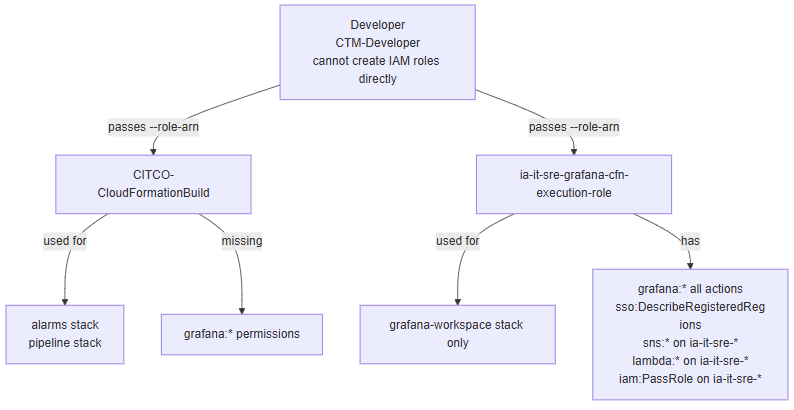
\includegraphics[width=0.85\textwidth]{figures/fig-IAM-Role-Architecture.png}
\caption[IAM Role Architecture --- Three-Role Model]{IAM Role Architecture --- Three-Role Model for Grafana AMG Deployment}
\label{fig:iam_role_model}
\end{figure}

\begin{itemize}
    \item \textbf{Metric Insights SQL}: I used CloudWatch Metric Insights SQL
          as the primary query language for
          multi-resource panels. This enabled
          SQL-like aggregation across all resources in a namespace with
          a single query, replacing the brittle \texttt{SEARCH()} expressions
          I had used in the earlier CloudWatch dashboard.
\end{itemize}

\subsubsection{Layer 2: Visualization Layer}

I built the Grafana AMG workspace with \textbf{17~dashboard rows} organized by
monitored service category. Table~\ref{tab:dashboard_rows} summarizes the
dashboard structure I implemented.

\begin{tabularx}{\textwidth}{@{\hspace{\tabcolsep}}>{\centering\arraybackslash}p{0.05\textwidth}>{\raggedright\arraybackslash}p{0.18\textwidth}>{\raggedright\arraybackslash}X@{\hspace{\tabcolsep}}}
\caption{Grafana AMG Dashboard --- Row Structure} \label{tab:dashboard_rows} \\
\hline
\rowcolor{smubrand}\textcolor{white}{\textbf{Row}} & \textcolor{white}{\textbf{Service}} & \textcolor{white}{\textbf{Panels and Metrics}} \\
\hline
\endfirsthead
\hline
\rowcolor{smubrand}\textcolor{white}{\textbf{Row}} & \textcolor{white}{\textbf{Service}} & \textcolor{white}{\textbf{Panels and Metrics}} \\
\hline
\endhead
\hline
\endfoot
\rowcolor{tablerowA} 1 & Health Overview & Color-coded stat tile per service (Lambda, SQS, MSK, EC2, ECR, EKS, ECS, RDS, DocumentDB, Redis, Neptune, OpenSearch); critical/warning alarm counts \\
\rowcolor{tablerowB} 2 & Performance Overview & Top-10 bargauge comparisons per service --- highest queue depth, Lambda errors, ECS CPU, Kafka consumer lag, Redis memory, etc. \\
\rowcolor{tablerowA} 3 & Lambda & Invocations, errors, throttles, concurrent executions, duration P50/P99; Logs Insights error panel \\
\rowcolor{tablerowB} 4 & SQS & Queue depth (\texttt{ApproximateNumberOfMessagesVisible}), oldest message age, DLQ depth \\
\rowcolor{tablerowA} 5 & MSK/Kafka & Consumer lag: \texttt{SumOffsetLag} and \texttt{EstimatedMaxTimeLag}; broker CPU, disk, messages in/out per second \\
\rowcolor{tablerowB} 6 & EC2 & CPU (avg/max), memory (CloudWatch Agent), network I/O, disk I/O, status checks \\
\rowcolor{tablerowA} 7 & ECR & Container image pull activity \\
\rowcolor{tablerowB} 8 & EKS & Kubernetes node and pod metrics \\
\rowcolor{tablerowA} 9 & ECS Services & CPU and memory utilization per cluster and service; Container Insights task-level metrics \\
\rowcolor{tablerowB} 10 & ECS Target Groups & ALB request throughput, response time P50/P95/P99, HTTP 5xx/4xx error counts \\
\rowcolor{tablerowA} 11 & RDS / Aurora & CPU, database connections, read/write latency, IOPS, freeable memory \\
\rowcolor{tablerowB} 12 & DocumentDB & CPU, disk queue depth, active connections, read/write latency, IOPS \\
\rowcolor{tablerowA} 13 & Redis / Valkey & Engine CPU (avg/max), memory, cache hit rate, replication lag, connections, latency \\
\rowcolor{tablerowB} 14 & Neptune DB & CPU, Gremlin/SPARQL errors, freeable memory, queue depth, network throughput \\
\rowcolor{tablerowA} 15 & OpenSearch & Cluster status (green/yellow/red), JVM heap pressure, indexing rate, search latency \\
\hline
\end{tabularx}

Figures~\ref{fig:grafana_overview}--\ref{fig:grafana_ecs} show live
screenshots from the Grafana AMG dashboard I deployed, demonstrating the
Health Overview, Lambda monitoring, and ECS monitoring rows I built.

\begin{figure}[htbp]
\centering
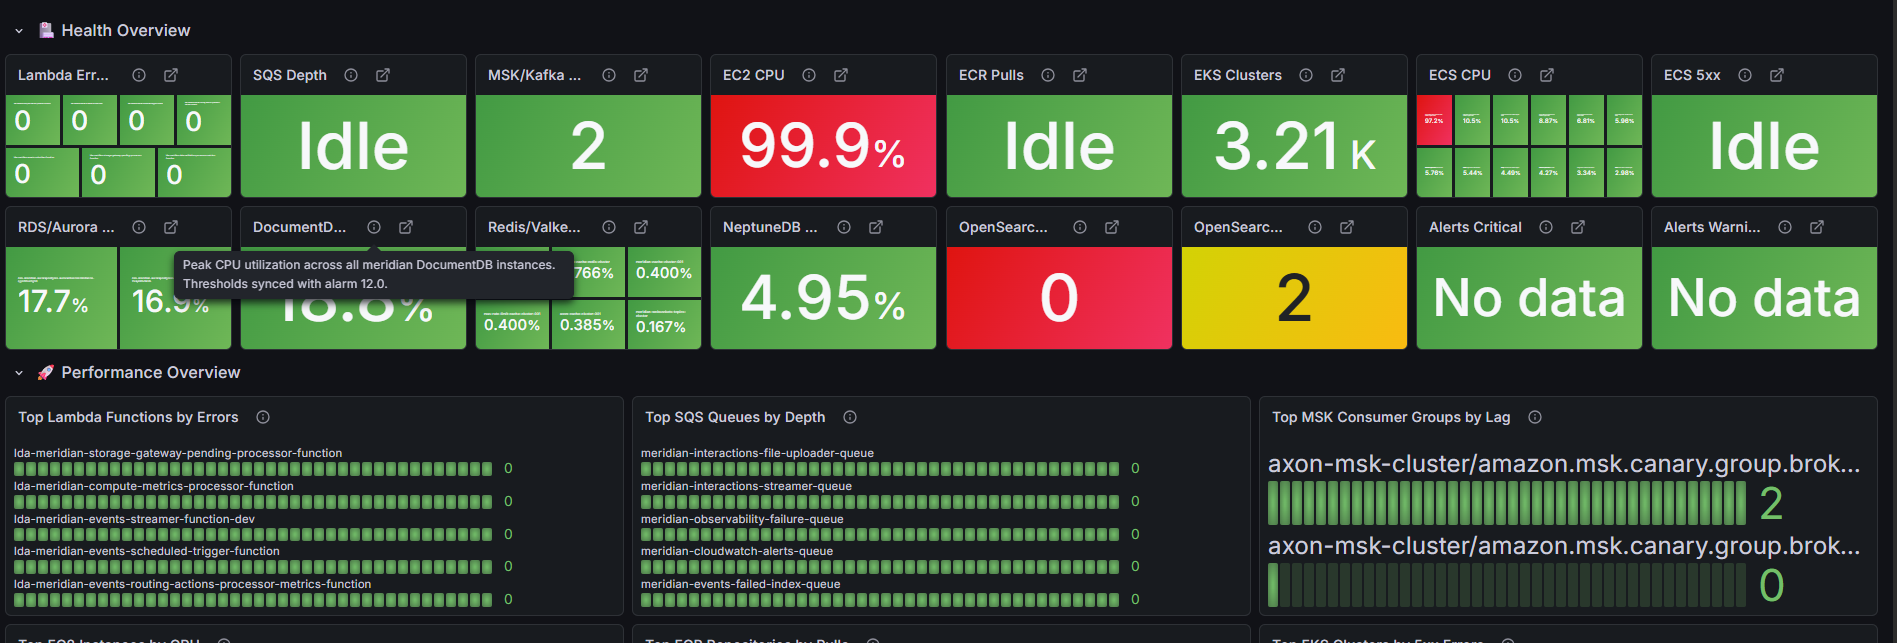
\includegraphics[width=0.95\textwidth]{figures/fig-grafana-overview-row.png}
\caption[Grafana AMG Dashboard --- Health Overview Row]{Grafana AMG Dashboard --- Health Overview Row (Live Screenshot)}
\label{fig:grafana_overview}
\end{figure}

\begin{figure}[htbp]
\centering
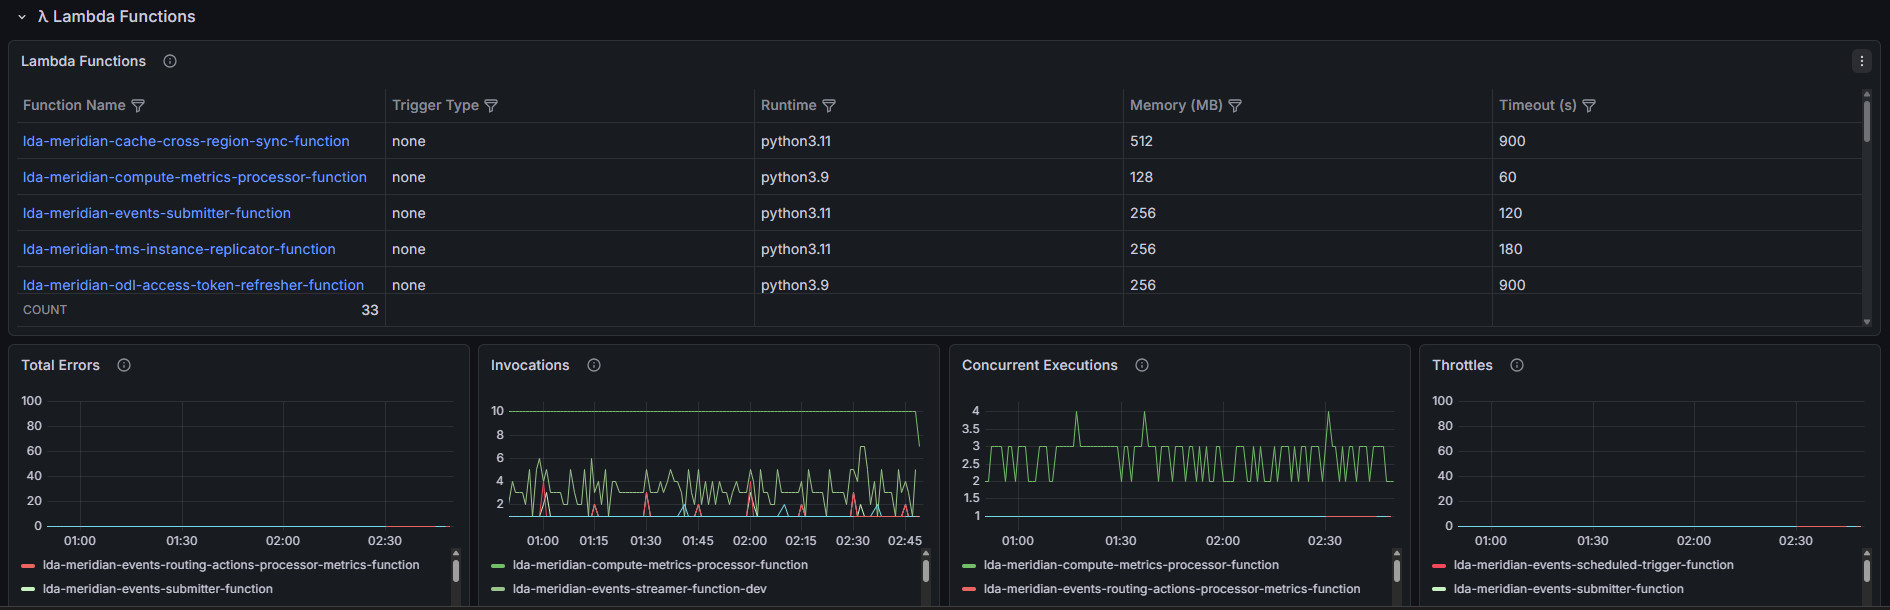
\includegraphics[width=0.95\textwidth]{figures/fig-grafana-lambda-row.png}
\caption[Grafana AMG Dashboard --- Lambda Monitoring Row]{Grafana AMG Dashboard --- Lambda Monitoring Row (Live Screenshot)}
\label{fig:grafana_lambda}
\end{figure}

The Lambda Monitoring Row (Figure~\ref{fig:grafana_lambda}) I built provides
real-time visibility into all Lambda functions across the selected
environment. The top table displays function names, trigger types,
runtime versions, memory allocations, and timeout configurations ---
enabling operators to identify misconfigured functions at a glance.
Below the table, I added four time-series panels tracking the four golden signals:
\textbf{Total Errors} (count of failed invocations), \textbf{Invocations}
(throughput), \textbf{Concurrent Executions} (saturation indicator), and
\textbf{Throttles} (capacity limit breaches). I added a color-coded legend below each panel
to enable drill-down to individual functions.

\begin{figure}[htbp]
\centering
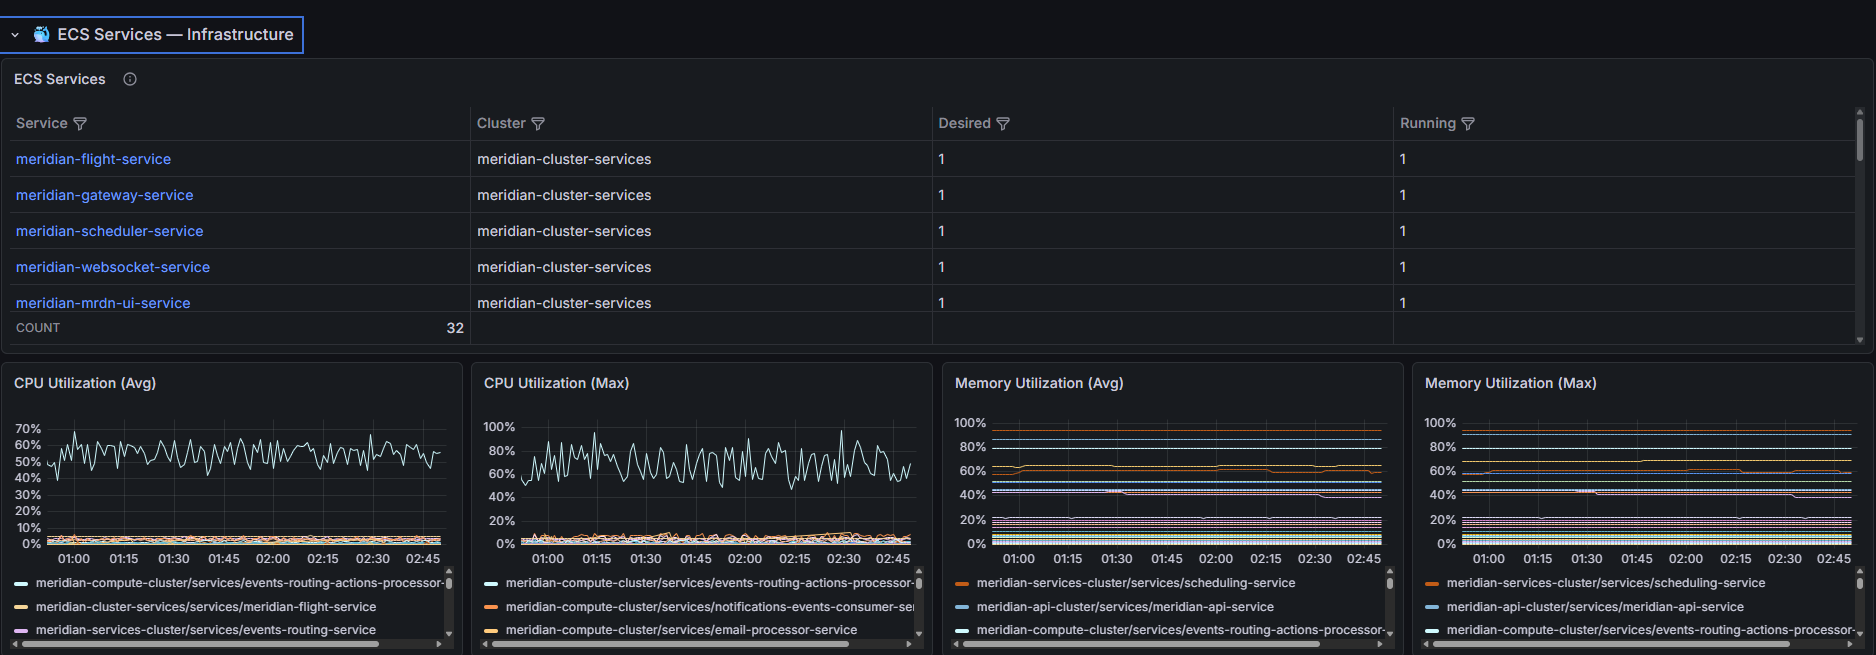
\includegraphics[width=0.95\textwidth]{figures/fig-grafana-ecs-row.png}
\caption[Grafana AMG Dashboard --- ECS Monitoring Row]{Grafana AMG Dashboard --- ECS Monitoring Row (Live Screenshot)}
\label{fig:grafana_ecs}
\end{figure}

The ECS Monitoring Row (Figure~\ref{fig:grafana_ecs}) I built surfaces
Container Insights metrics for all ECS services in the selected cluster.
I added a service table showing cluster assignment, desired count, and running
count --- highlighting any discrepancies that indicate failed deployments
or scaling issues. I also added four time-series panels displaying CPU and memory
utilization (both average and maximum) across all tasks, enabling
operators to identify resource saturation before it impacts service
availability. This row was particularly valuable for monitoring the
Meridian ECS services, where memory pressure had previously gone
undetected until task failures occurred.

\textbf{Grafana Template Variables.}
I implemented environment-level filtering through three Grafana
template variables backed by CloudWatch dimension-value queries:

\begin{itemize}
    \item \texttt{\$budget\_code} --- filters all panels to a specific
          environment (\texttt{rpacfs1}, \texttt{ia-bpo}, \texttt{meridian},
          \texttt{citcoworks}, \texttt{automationhub}). Backed by a
          CloudWatch \texttt{ListMetrics} call enumerating distinct
          budget\_code tag values.

    \item \texttt{\$ecs\_cluster} --- filters ECS panels to a specific
          cluster. Backed by a \texttt{dimension\_values()} query on
          the \texttt{ECS/ContainerInsights} namespace.

    \item \texttt{\$lambda\_function} --- filters Lambda panels to a
          specific function. Backed by a \texttt{dimension\_values()}
          query on the \texttt{AWS/Lambda} namespace.
\end{itemize}

When a user selects a value from any variable, all panels that reference
that variable re-execute their queries with the selected filter applied,
scoping the entire dashboard to a single environment or
resource. I designed it this way to eliminate the need to maintain separate dashboards per
platform.

\textbf{CloudWatch Metric Insights SQL: Architecture Pattern.}
CloudWatch Metric Insights SQL is the key architectural pattern I adopted to
enable per-resource drill-down across large fleets within a single query.
I used the standard \texttt{SELECT ... FROM ... GROUP BY} form to return
metrics for each resource as a separate time series, covering all resources
without requiring one panel per function. I used the \texttt{WHERE} clause to
filter by tag or dimension and scope results to specific platforms.

\paragraph{Percentile Limitation and Workaround.}
A fundamental constraint of Metric Insights SQL is that the
\texttt{GROUP BY} mode only supports the aggregate functions
\texttt{AVG}, \texttt{SUM}, \texttt{MIN}, and \texttt{MAX}. Percentile
statistics (p50, p95, p99) are \emph{not
available} in \texttt{GROUP BY} mode. This is a CloudWatch API limitation,
not a Grafana limitation.

For panels requiring true latency percentiles, the workaround is to use
the \emph{standard CloudWatch metrics} query mode with a wildcard
dimension value (e.g., \texttt{FunctionName: ["*"]}). This returns
individual time series for each function that has emitted metrics within
the selected time window. The tradeoff is that only recently active functions
appear --- the same ``visibility gap'' limitation noted for \texttt{SEARCH()}.
For the Lambda duration P50/P95 panels, I accepted this tradeoff:
a function that has not been invoked recently has no meaningful latency
distribution to display.

\subsubsection{Layer 3: Alerting Layer}

I provisioned \textbf{dynamic CloudWatch alarms} across all monitored
platforms, each connected to an SNS topic that routes notifications to
the IA-SRE team's email distribution list. Alarm categories include:

\begin{itemize}
    \item \textbf{Lambda alarms}: Error rate exceeding 1\% over a
          5-minute rolling window; throttle count exceeding threshold;
          concurrent execution count approaching account limit.

    \item \textbf{ECS alarms}: CPU utilization sustained above 80\%
          over a 5-minute evaluation period; task desired count $\neq$
          running count (task failure detection).

    \item \textbf{MSK alarms}: \texttt{EstimatedMaxTimeLag} exceeding
          10,000~messages on any consumer group. This alarm directly
          addresses the Meridian Incident: it would have fired within
          minutes of the lag beginning to build, compared to the 3.5-hour
          detection gap that occurred under the reactive model.
\end{itemize}

\begin{itemize}
    \item \textbf{SQS alarms}: Queue depth exceeding configurable
          threshold per queue; \texttt{ApproximateAgeOfOldestMessage}
          exceeding 1~hour (configurable per SLA).

    \item \textbf{Composite alarms}: Platform-level health signals that
          aggregate per-service alarm states into a single
          OK/ALARM indicator per budget\_code environment.
\end{itemize}

\subsubsection{Layer 4: Infrastructure-as-Code Provisioner}

The IaC layer is a \textbf{Lambda-backed CloudFormation provisioner}
I deployed via AWS SAM. I designed it to address a specific scaling
constraint: with 119~Lambda functions, a static CloudFormation template
defining one alarm per function would contain $119 \times (\text{alarm
types per function})$ resources, rapidly approaching the CloudFormation
500-resource-per-stack limit.

I resolved this by making the provisioner \emph{dynamically discover} the
current function fleet at deploy time and synthesize alarm resources
programmatically:

\begin{enumerate}
    \item The provisioner Lambda function I wrote is invoked by a CloudFormation
          custom resource on every \texttt{samconfig.toml} deploy.

    \item It reads parameterized CloudFormation YAML templates I stored in an
          S3 bucket (see Section~\ref{sec:decision_secrets_s3}).

    \item For each template (Lambda alarms, ECS alarms, SQS alarms, MSK
          alarms), it calls the relevant AWS discovery API to enumerate
          all current resources in the specified platform.

    \item It synthesizes CloudFormation \texttt{AWS::CloudWatch::Alarm}
          resource blocks for each discovered resource and passes the
          generated template to CloudFormation for stack deployment.

    \item I deployed four CloudFormation stacks on
          \textbf{May~11, 2026}: \texttt{ia-sre-lambda-alarms},
          \texttt{ia-sre-ecs-alarms}, \texttt{ia-sre-sqs-alarms}, and
          \texttt{ia-sre-msk-alarms}.
\end{enumerate}

I wrote a \texttt{samconfig.toml} with environment-specific parameter files
to enable reuse across DEV, UAT, and PROD without code changes. I externalized the budget
code, alarm thresholds, and SNS topic ARN as SAM parameters, satisfying NFR5 (multi-environment reuse).

Figure~\ref{fig:alarm_notification_flow} illustrates the alarm notification
flow from CloudWatch alarm state change through SNS topic fan-out to the
IA-SRE team's email distribution list.

\begin{figure}[htbp]
\centering
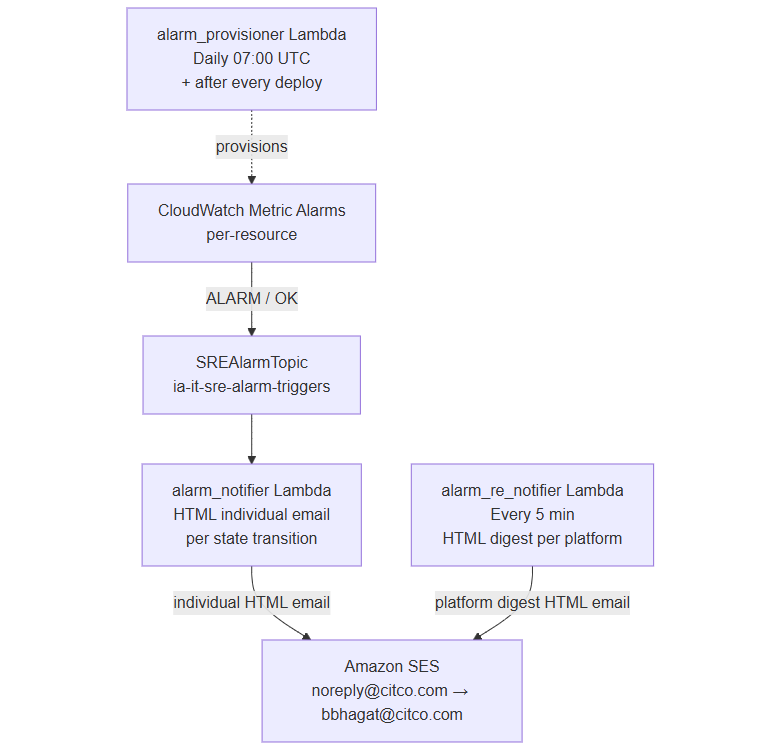
\includegraphics[width=0.85\textwidth]{figures/fig-alarm-notification-flow.png}
\caption[Alarm Notification Flow --- CloudWatch to SNS]{Alarm Notification Flow --- CloudWatch to SNS to Email Distribution}
\label{fig:alarm_notification_flow}
\end{figure}

Figure~\ref{fig:amg_deployment_flow} shows the CodePipeline CI/CD deployment
flow that delivers all stacks across the three environments.

\begin{figure}[htbp]
\centering
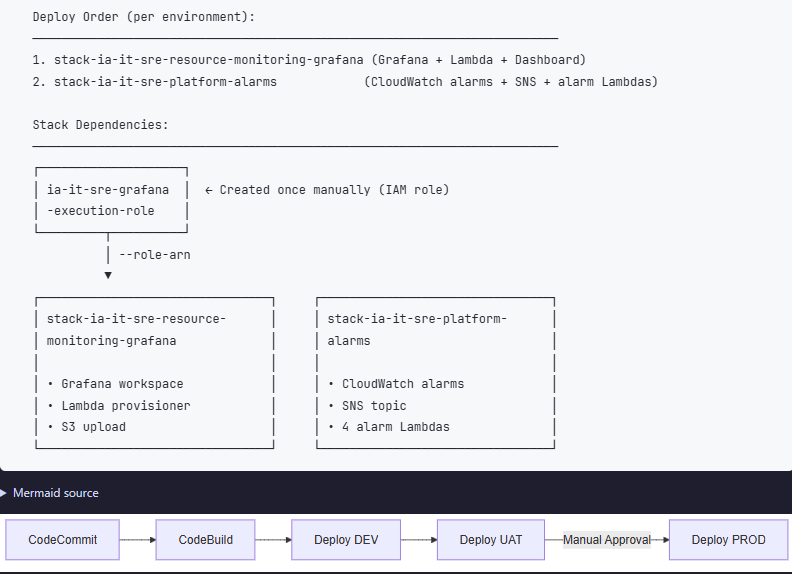
\includegraphics[width=0.95\textwidth]{figures/fig-amg-deployment-flow.png}
\caption[CI/CD Deployment Pipeline --- CodeCommit to AMG]{CI/CD Deployment Pipeline --- CodeCommit to AMG Deployment Flow}
\label{fig:amg_deployment_flow}
\end{figure}

\subsection{Grafana Version Upgrade: Architectural Resilience Test}

On \textbf{May~13, 2026} --- two days after my initial infrastructure
deployment --- the Grafana AMG workspace was upgraded from version
\textbf{10.4 to 12.4}. This was a major version migration that
constituted an unplanned but highly informative architectural resilience
test for the dashboard I had built.

The upgrade introduced breaking changes in two areas:

\begin{itemize}
    \item \textbf{CloudWatch Metric Insights SQL editor}: The query
          syntax editor in Grafana 12.4 changed the way SQL expressions
          were associated with panel targets. All SQL panels required
          migration to the updated CloudWatch query model.

    \item \textbf{Variable interpolation}: Template variable syntax
          in panel queries changed between versions, causing several
          \texttt{\$budget\_code} and \texttt{\$ecs\_cluster} references
          to fail to resolve correctly after the upgrade.
\end{itemize}

I resolved this through a systematic audit of all panels to identify
affected queries. The migration reinforced a key design principle
I documented as NFR6: \textbf{use only standard CloudWatch plugin queries
and avoid AMG-version-specific syntax}. I migrated all panel queries
to the stable Grafana 12.4 CloudWatch query model, and the workspace has
remained stable through subsequent Grafana patch releases.

\subsection{X-Ray Distributed Tracing (PoC)}

As part of the observability stack I built, I integrated AWS X-Ray tracing to
provide distributed trace visibility across the IA platform. The X-Ray
integration I configured enables service map visualization and trace waterfall
analysis --- capabilities that contribute to the 60\% Dynatrace parity
achieved by the CloudWatch + Grafana + X-Ray stack I assembled (see
Section~\ref{sec:dynatrace_parity}).

Figure~\ref{fig:xray_service_map} shows the X-Ray service map displaying
the trace topology for the RPA-LLM platform, illustrating how requests
flow through Lambda functions, external APIs, and AWS services.

\begin{figure}[htbp]
\centering
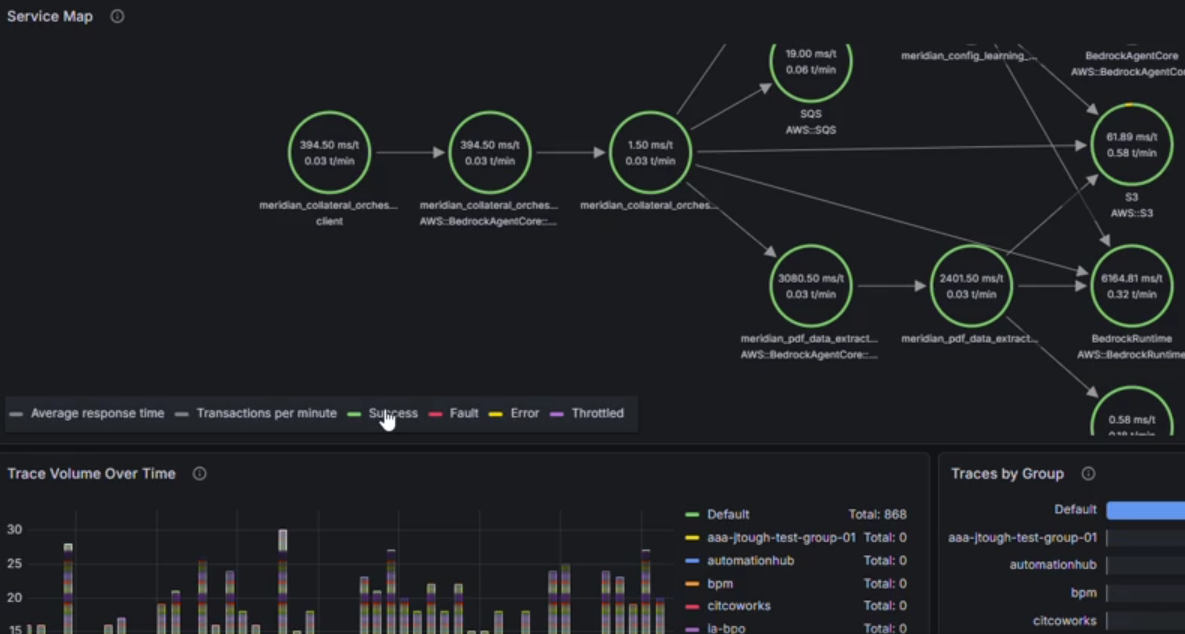
\includegraphics[width=0.95\textwidth]{figures/fig-xray-service-map.png}
\caption[AWS X-Ray Service Map --- Distributed Trace Topology]{AWS X-Ray Service Map --- Distributed Trace Topology (Live Screenshot)}
\label{fig:xray_service_map}
\end{figure}

The X-Ray integration delivers three key capabilities:

\begin{itemize}
    \item \textbf{Service Map}: Visual representation of service
          dependencies and request flow, enabling rapid identification
          of bottlenecks and failure points.
    \item \textbf{Trace Waterfall}: Detailed timing breakdown for
          individual requests, showing latency contribution from each
          service in the call chain.
    \item \textbf{Error Analysis}: Automatic capture of exceptions and
          error responses with stack traces, correlated to specific
          trace segments.
\end{itemize}

X-Ray tracing is currently enabled in DEV environment only; I am awaiting senior approval for UAT and PROD enablement due to the additional CloudWatch costs associated with trace segment storage.

\FloatBarrier

\section{Work Stream 3: IA Resources Inventory API}
\label{sec:inventory_api}


I built a \textbf{Flask REST API} for programmatic discovery
of all IA platform cloud resources. I created the
\texttt{ia-sre-resources-inventory} repository and scaffolded the project on
Jun~11, 2026; I brought it to production-ready state with 562~automated
tests and 99\%~code coverage.

\subsection{Technology Stack}

\begin{itemize}
    \item \textbf{Language}: Python~3, \texttt{flask[async]} for async
          route handlers
    \item \textbf{AWS SDK}: boto3 for all resource discovery
    \item \textbf{Validation}: Pydantic response models (type-safe
          \texttt{Resource} dataclass with fields: name,
          type, \texttt{budget\_code}, tags,
          arn)
    \item \textbf{Deployment}: AWS Lambda via serverless-wsgi
          adapter
    \item \textbf{Testing}: pytest + Hypothesis
          (property-based tests)
\end{itemize}

\subsection{Discoverer Registry Pattern}

My core architectural contribution in the inventory API is the
\textbf{Discoverer Registry pattern}. Rather than routing resource
discovery logic through a monolithic handler, I built a
registry that maps \texttt{(resource\_type, budget\_code)} tuples to
concrete discoverer classes. Each discoverer implements a single abstract
method \texttt{async def discover() -> List[Resource]}. Adding support for a
new platform or resource type requires implementing one class and
registering one entry --- zero changes to routing, serialization, or
test infrastructure.

\subsection{API Endpoints}

\begin{tabularx}{\textwidth}{@{\hspace{\tabcolsep}}>{\raggedright\arraybackslash}p{0.28\textwidth}>{\raggedright\arraybackslash}X@{\hspace{\tabcolsep}}}
\caption{IA Resources Inventory API --- Endpoint Summary} \label{tab:api_endpoints} \\
\hline
\rowcolor{smubrand}\textcolor{white}{\textbf{Endpoint}} & \textcolor{white}{\textbf{Description}} \\
\hline
\endfirsthead
\hline
\rowcolor{smubrand}\textcolor{white}{\textbf{Endpoint}} & \textcolor{white}{\textbf{Description}} \\
\hline
\endhead
\hline
\endfoot
\rowcolor{tablerowA} \texttt{GET /api/v1/lambda} & All Lambda functions; optional
  \texttt{?budget\_code=rpacfs1} filter \\
\rowcolor{tablerowB} \texttt{GET /api/v1/ecs} & All ECS clusters across all platforms \\
\rowcolor{tablerowA} \texttt{GET /api/v1/ec2} & All EC2 instances (tag-based discovery) \\
\rowcolor{tablerowB} \texttt{GET /api/v1/secrets} & Secrets Manager secrets inventory \\
\rowcolor{tablerowA} \texttt{GET /api/v1/s3} & S3 buckets per budget\_code \\
\rowcolor{tablerowB} \texttt{GET /api/v1/health} & Health check --- returns 200 OK \\
\hline
\end{tabularx}

\subsection{Tag-Based Discovery and the Two-Stage Filter}

The most technically interesting discovery challenge I encountered was the
\texttt{citcoworks} and \texttt{meridian} tag ambiguity. Both
environments share the AWS tag value \textbf{"Shared Cloud Artifacts"}
for the budget\_code dimension --- a legacy of the two platforms
being onboarded before the IA team established per-platform
budget\_code uniqueness requirements. A naive
budget\_code lookup would conflate resources from two operationally
distinct environments.

Figure~\ref{fig:grafana_inventory_integration} shows how the Inventory API integrates
with the Grafana AMG dashboard --- the cache-refresh Lambda writes S3 snapshots and
publishes CloudWatch metrics, which Grafana reads via template variables and Metric
Insights SQL panels.

\begin{figure}[htbp]
\centering
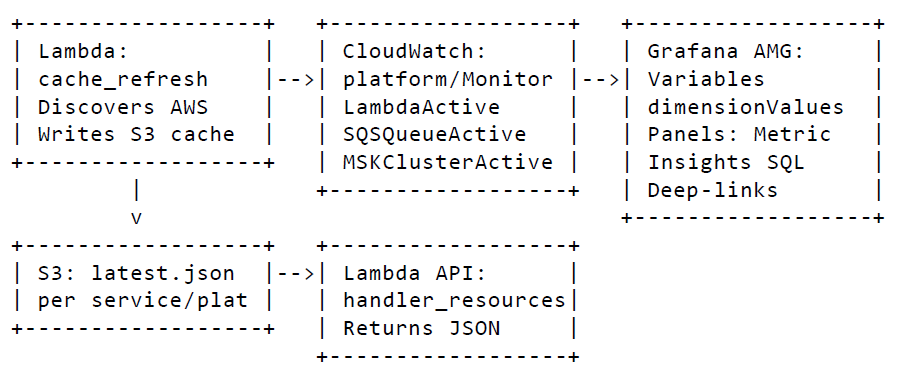
\includegraphics[width=0.92\textwidth]{figures/fig-grafana_inventory_integration.png}
\caption{Inventory API --- Grafana AMG Integration}
\label{fig:grafana_inventory_integration}
\end{figure}

I implemented a \textbf{two-stage filter} in both the
\texttt{CitcoWorksECSDiscoverer} and \texttt{MeridianECSDiscoverer}.
Stage~1 filters by budget\_code (which is shared between both platforms),
then Stage~2 uses the AppName tag to discriminate Meridian resources
from CitcoWorks resources.

I designated the AppName tag as the \textbf{mandatory secondary
discriminator} for all resources in the \textbf{``Shared Cloud Artifacts''}
budget\_code environments. Any new resource added to either environment
without the correct AppName tag will be invisible to the
inventory API. I mitigated this risk with a tag compliance CloudWatch
alarm that fires if new ECS services or Lambda functions lack the
required tags.

Figure~\ref{fig:resource_discovery_flow} illustrates the complete
resource discovery flow, showing how the API routes requests through
the discoverer registry and applies the two-stage filter for ambiguous
budget\_codes.

\begin{figure}[htbp]
\centering
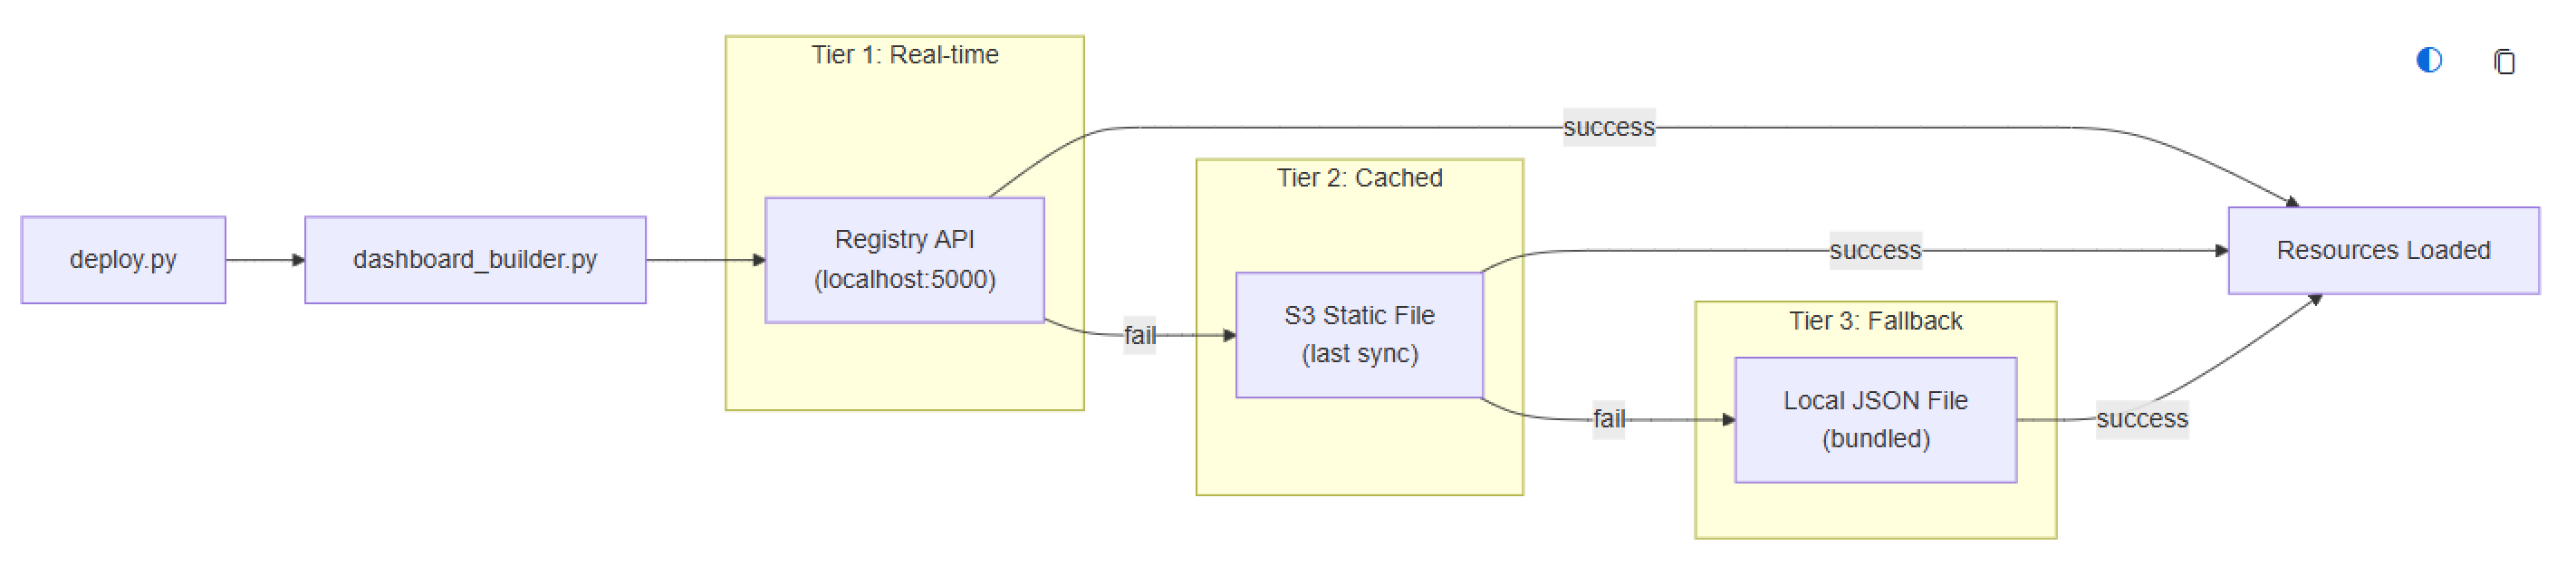
\includegraphics[width=0.85\textwidth]{figures/fig-resource-discovery-flow.png}
\caption[Resource Discovery Flow --- Two-Stage Filter]{Resource Discovery Flow --- Discoverer Registry and Two-Stage Filter}
\label{fig:resource_discovery_flow}
\end{figure}

\subsection{Async Architecture}

I built the API using \texttt{flask[async]} with async route handlers.
Each handler aggregates boto3 calls concurrently using
\texttt{asyncio.gather()}, reducing total API latency by parallelizing
the AWS API calls within a single request. All matching discoverers run
concurrently rather than sequentially, reducing API response time from
the sum of all boto3 call latencies to the latency of the single slowest
call --- consistently keeping the API within the 10-second NFR3 target.

\subsection{Test Strategy}

My test suite for the inventory API achieves \textbf{99\%~code coverage}:

\begin{itemize}
    \item \textbf{Unit tests}: Each discoverer class tested in isolation
          with mocked boto3 clients. Verifies correct tag filtering,
          pagination handling, and \texttt{Resource} object construction.

    \item \textbf{Integration tests}: Full Flask test client hitting
          all REST endpoints. Verifies routing, serialization, and
          error response format.

    \item \textbf{Property-based tests (Hypothesis)}: Tag-parsing logic,
          registry dispatch, and Pydantic response serialization tested
          with randomly generated inputs. Verifies that the two-stage
          filter never returns a \texttt{meridian} resource when
          \texttt{budget\_code=citcoworks} is specified, regardless of
          what combination of tag values is present.

    \item \textbf{Edge case tests}: Malformed tags, empty budget\_code
          environments, boto3 pagination edge cases (empty pages,
          single-page results, maximum page sizes).
\end{itemize}

\FloatBarrier

\section{Work Stream 4: RPA Production Support}
\label{sec:rpa_production_support}


Throughout the co-op placement I participated in dedicated RPA production support
rotations as part of the IA team's \textbf{Follow-the-Sun model}. I operated within a three-tier support structure:

\begin{itemize}
    \item \textbf{L1 --- Ask Citco RPA} (Work Stream~5): The LLM-powered
          self-service chatbot I also worked on, which answers first-line queries from RPA
          operators about process status, procedures, and Legal Entity assignments.
    \item \textbf{L2 --- Innovation IT Support} (Work Stream~4): The
          human-staffed Follow-the-Sun rotation I participated in, covering Manila (APAC),
          Dublin (EMEA), and Halifax (NA) shifts. At L2 I handled Service Desk
          tickets that L1 could not resolve, performing triage, investigation,
          and resolution or escalation.
    \item \textbf{L3 --- SRE} (our team): The escalation tier for
          infrastructure-level incidents requiring cloud access, code-level
          fixes, or platform changes beyond L2 scope.
\end{itemize}

I held the North America L2 slot (11~AM--7~PM~EST) on a weekly rotation among the four
NA-based SRE team members, serving as the primary contact for RPA incidents during that window. This was
not project work with JIRA tickets --- it was ongoing operational
responsibility with Service Desk tickets, email triage, and ad-hoc troubleshooting.

\subsection{Support Rotation Structure}

Each support week followed a consistent daily rhythm:

\begin{itemize}
    \item \textbf{Shift start (11~AM~EST)}: Review the Confluence handover
          log from the Manila shift to pick up carried-over items or
          approaching SLA breaches. Check open tickets in the SD Portal,
          Innovation IT email inbox, \texttt{IA\_INCIDENTS} distribution
          list, and Teams notifications.

    \item \textbf{During shift}: Monitor VPL queue health (5~PM~EST daily
          checkpoint), respond to escalations from Dublin/London business
          teams, triage incoming tickets, and coordinate with developers
          when code-level fixes are required.

    \item \textbf{Shift end (7~PM~EST)}: Update the Confluence handover log
          with ticket status, any pending actions, and context for the
          next shift (Manila).
\end{itemize}

\subsection{Support Weeks Completed}

I completed four full support rotations during the co-op placement:

\begin{itemize}
    \item \textbf{Week 8} (May~4--8): First rotation. Familiarization with
          SD Portal, VPL queue monitoring, and the escalation ladder.
          Shadowed Mr.\ Leung on Corporate Actions ticket triage.

    \item \textbf{Week 12} (Jun~1--5): MESO hotfix week. Encountered
          MESO ECS autoscaling incident (ECS autoscaling gap) during routine monitoring ---
          this led to a code fix, not just ticket resolution.

    \item \textbf{Week 20} (Jul~27--31): VPL GTL booking error incident (VPL Pricing GTL booking
          error). Coordinated with the business team on NAV impact
          assessment. Also handled routine queue monitoring and ticket
          triage.

    \item \textbf{Week 23} (Aug~17--21): Final rotation. Lighter ticket
          volume; used remaining time for report writing and KT preparation.
\end{itemize}

\subsection{Notable Incidents Handled}

While most support work involved routine ticket triage and queue monitoring,
several incidents required deeper investigation or code-level fixes:

\begin{itemize}
    \item \textbf{CAIS Deadline Pipeline Hotfix:} The CAIS Deadline bot --- which uploads Standard Allocation Sheets to the PDS database and downloads deadline pricing reports --- failed with
          \texttt{SMBAuthenticationError: SpnegoError}. Seven-hour
          investigation traced to Secrets Manager credential rotation
          leaving empty values cached at module import time. Hotfix
          added fail-fast validation. Filing completed before regulatory
          deadline.

    \item \textbf{MESO ECS}: Tasks stuck, not autoscaling.
          Root cause: ECS service autoscaling policy was unconfigured.
          Fixed the scaling policy and added an ECS \texttt{SaturationAlarm}
          to the dashboard alarm set.

    \item \textbf{MESO Critical}: INNOCAP and SAMLMOS funds
          stuck in queue with no Lambda heartbeat. Manually retriggered
          the \texttt{ia\_meso\_process} pipeline. Processing completed
          approximately 2~hours after escalation.

    \item \textbf{VPL IPV}: \AE xeo pricing window
          \texttt{CheckpointException} in UiPath --- bot exhausted its
          retry budget waiting for a dynamic UI element. Estimated 16~hours
          for selector resilience fix; escalated to the development team.
\end{itemize}

\subsection{Value of Support Rotation for SRE Work}

The support rotation was not separate from the SRE observability work ---
it was \emph{complementary}. Several incidents I encountered during support
weeks directly influenced the dashboard and alarm design:

\begin{itemize}
    \item The MESO ECS incident led to adding the
          \texttt{ECS\_CPUSaturation} alarm to the Grafana dashboard.

    \item The CAIS Deadline credential failure reinforced the importance
          of fail-fast validation patterns documented in the Challenges
          chapter.

    \item VPL queue monitoring during support shifts provided real-world
          validation of the SQS dashboard panels and queue depth alarms.
\end{itemize}

When ticket volume was low, I used remaining support shift time for
development work on the dashboard, inventory API, or documentation ---
maintaining productivity while remaining available for escalations.

\FloatBarrier

\section{Work Stream 5: RPA LLM Agent --- Ask Citco RPA}
\label{sec:rpa_llm_agent}


During Week~21 I engaged with a parallel work stream outside the SRE
monitoring scope: the \textbf{Ask Citco RPA} support chatbot, implemented
across two CodeCommit repositories (\texttt{ml-rpa-status-llm-agent} and
\texttt{core-smart-rpa-llm-ecr-image}). I started with a research
and documentation task but expanded into production bug-fixing after my log
analysis revealed critical reliability failures.

\subsection{System Architecture}

The chatbot is a \textbf{Retrieval-Augmented Generation (RAG)} pipeline
built on Amazon Bedrock, designed to answer RPA operator queries about
process status, procedures, and Legal Entity assignments without requiring
developers to be on-call for routine questions. I studied the architecture
in depth as part of my onboarding to the codebase before beginning my
own contributions.

\begin{figure}[htbp]
\centering
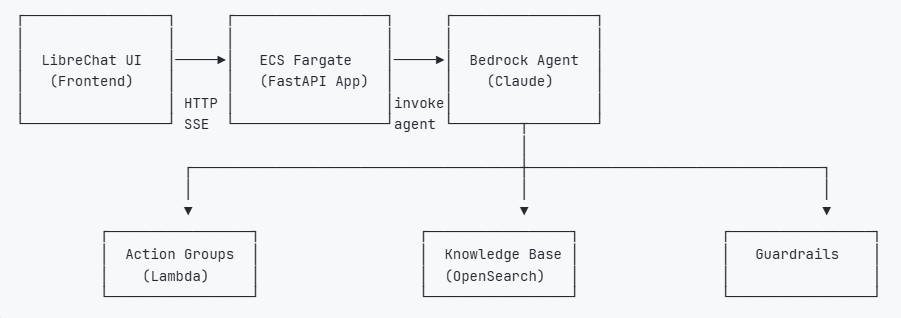
\includegraphics[width=0.90\textwidth]{figures/fig-rpa-llm-architecture.png}
\caption{Ask Citco RPA --- RAG Architecture}
\label{fig:rpa_llm_arch}
\end{figure}

The \textbf{ECS Fargate} layer runs the FastAPI container, authenticates
users via LDAP (checking \texttt{rpa\_support\_agent\_user} AD group), invokes
the Bedrock agent, and streams responses back in OpenAI SSE format. The
\textbf{Bedrock Agent} (Claude) orchestrates between action groups and
the Knowledge Base depending on the query type: process status queries
hit the Event Service Lambda; procedural questions retrieve chunks from
OpenSearch via hybrid vector and keyword search.

\subsection{Knowledge Base Pipeline}

I documented and analyzed the KB ingestion pipeline, which I found runs daily in two stages.
I traced the full flow to understand how to improve it:

\begin{enumerate}
    \item \textbf{12:00 UTC --- \texttt{IRCOEKBExtractLambda}}: I found this function syncs
          49 SharePoint IRCOEKB wiki libraries ($\sim$5,000 pages) to S3
          as plain-text files with SharePoint metadata preserved.
    \item \textbf{14:00 UTC --- \texttt{RPALLMKBIngestionFunction}}: This triggers
          Bedrock KB ingestion, which chunks (hierarchical: 1,200 token
          parent / 300 token child), embeds (1024-dim), and indexes into
          OpenSearch Serverless (FAISS/HNSW, L2 distance).
\end{enumerate}

I also reviewed the static document upload script (\texttt{scripts/upload\_kb\_content.py}),
which compares content hashes before writing to S3 to provide idempotent uploads.

\subsection{Production Reliability Issues Identified and Fixed}

I began my work on this codebase with CloudWatch log analysis. My analysis of
\textbf{93 days of production logs} (May~5 -- August~5, 2026; 148 Lambda
runs) revealed a critical reliability failure in the KB sync:

\begin{itemize}
    \item \textbf{52\% timeout rate on \texttt{IRCOEKBExtractLambda}.}
          77 of 148 production runs hit the 300-second Lambda timeout.
          June 2026 was the worst month at 71\% timeout rate. Average
          run duration was 291 seconds --- every run within 36 seconds of
          the limit. When the Lambda timed out, the Knowledge Base was
          incomplete for that day: pages not yet uploaded when the timeout
          fired were missing from the KB until the next successful run.

    \item \textbf{Root cause: unconditional full re-upload.}
          The original code re-uploaded all $\sim$980 pages on every daily
          run regardless of whether content had changed. The
          \texttt{KB Articles} library alone (1,266 pages at $\sim$220ms
          per S3 \texttt{head\_object} call) required 278 seconds just
          for change detection I/O.
\end{itemize}

I implemented a two-phase hybrid sync (\textbf{v1.1.x + v1.1.18}) that
reduced steady-state run time from 291 seconds average to approximately
\textbf{25 seconds}:

\begin{enumerate}
    \item \textbf{Phase 1 --- Library-level change detection ($\sim$25s
          for all 49 libraries).} One lightweight ALB call per library
          using a SharePoint \texttt{filter=Modified gt \{last\_synced\_at\}}
          query. Zero results means the entire library is unchanged and
          is skipped with no further I/O.
    \item \textbf{Phase 2 --- Conditional sync.} Only changed libraries
          are processed. Sequential if five or fewer changed; parallel
          via \texttt{ThreadPoolExecutor(max\_workers=3)} if more than
          five changed.
    \item \textbf{Per-page idempotency.} Within each synced library,
          each page's SharePoint \texttt{Modified} timestamp is compared
          to the \texttt{sp-modified} field stored in S3 object metadata.
          Unchanged pages skip HTML extraction and S3 upload entirely.
\end{enumerate}

Beyond the KB sync, log analysis also surfaced seven additional
production bugs fixed across versions v1.1.1--v1.1.32:

\begin{itemize}
    \item \textbf{OpenSearch silent delete} (v1.1.1): index creation
          failure silently deleted the index and reported CloudFormation
          SUCCESS. Fixed with proper exception handling and idempotency
          check.
    \item \textbf{Fire-and-forget Lambda pattern}: \texttt{EventStoreExtractLambda}
          and \texttt{ClientFundMappingLambda} always reported SUCCESS
          regardless of actual outcome due to incorrect exception class
          references (\texttt{boto3.exceptions.BotoError} does not exist).
    \item \textbf{Athena SSE encryption inconsistency}: queries used
          \texttt{SSE\_S3} instead of \texttt{SSE\_KMS} in some Lambdas.
    \item \textbf{Athena race condition}: \texttt{MSCK REPAIR TABLE}
          executed immediately after \texttt{CREATE TABLE} without
          waiting for completion.
    \item \textbf{SSL verification disabled}: BPM API calls used
          \texttt{verify=False}.
\end{itemize}

\paragraph{Knowledge Base Enrichment.}
As part of the RPA LLM Agent work, I uploaded the NavChecklist process documentation
PDFs (\textit{Architecture -- NAV CHECKLIST.pdf}, \textit{FAQ -- NAV
CHECKLIST.pdf}) to the KB S3 bucket under
\texttt{RPA Processes/NAV Checklist/} using the idempotent upload
script. These documents --- describing the NAV calculation checklist
process flow --- are now indexed in the production Knowledge Base and
searchable by the chatbot.

\subsection{Code Quality and Engineering Improvements}

Alongside the bug fixes, I delivered the following engineering quality
improvements to bring the codebase in line with IA Best Practice
guidelines (pending dev approval gate):

\begin{itemize}
    \item \textbf{Module refactor}: the 1,140-line monolithic
          \texttt{function.py} split into 8 focused modules
          (\texttt{handler.py}, \texttt{event\_service\_api.py},
          \texttt{secrets.py}, \texttt{project\_lookup.py}, etc.)
    \item \textbf{structlog migration}: replaced \texttt{print()} and
          root logger across all 11 Lambda functions with structlog
          structured logging
    \item \textbf{Type hints and docstrings}: PEP~484 type hints and
          Google-style docstrings added to all functions and classes
    \item \textbf{Test suite}: Comprehensive unit tests at 99\% code coverage
          (v1.1.x series)
    \item \textbf{Pydantic models}: Databricks API response and BPM
          API response wrapped in Pydantic validation models
    \item \textbf{Kill switch}: SSM Parameter Store kill switch
          (RUN/STOP) implemented across IRCOEKB, Event Store, and Mapping Lambdas
    \item \textbf{X-Ray tracing}: AWS Lambda Powertools Tracer
          instrumented on all functions (enabled in DEV; pending approval
          for UAT/PROD)
\end{itemize}

Versions v1.1.1 through v1.1.32 were released during August~3--20, 2026.

\subsection{Proposed: Hybrid Graph-RAG Architecture}

During my codebase analysis I identified a structural limitation of
the current flat-vector RAG approach for the Citco RPA domain. The
entities in this domain are highly relational: clients have funds, funds
run specific processes, processes execute on either Blue Prism or UiPath,
and each platform has its own operational knowledge base. A standard
vector similarity search treats all these entities as independent text
chunks, losing the relational structure.

I propose a \textbf{Hybrid Graph-RAG} enhancement: adding Amazon Neptune
as a graph layer alongside the existing OpenSearch vector store. I would model the entity relationship network (client--fund--process--platform)
as a graph, enabling the Bedrock agent to traverse relationships for multi-hop queries
(\textit{``Which Blue Prism processes handle FX Closeouts for client X?''}),
then retrieve dense context from the vector KB for the identified process
entities. The dual-path retrieval I am proposing would improve answer accuracy for
complex operational queries while maintaining the existing RAG pipeline
for straightforward procedural lookups. I will submit this proposal
as a formal follow-on work item.

\FloatBarrier

\section{Work Stream 6: Citco Enterprise Custom UI Dashboards}
\label{sec:enterprise_ui_dashboards}


During this co-op placement I began extending the existing
\texttt{ia-config-portal} application with two new dashboard pages.
I completed a comprehensive \textbf{architectural implementation plan}
(Infrastructure Monitoring Dashboard-IMPLEMENTATION-PLAN.md) and started
initial implementation. I am continuing this development during the co-op
extension period (Sep--Dec~2026).

\subsection{Planning Document Deliverable}

The primary deliverable I produced for this work stream is a comprehensive
865-line implementation plan that I wrote documenting:

\begin{itemize}
    \item \textbf{Gap analysis}: I identified and documented 45 Grafana AMG limitations
          with severity ratings, determining which gaps justify a
          custom UI solution.

    \item \textbf{Technology stack decisions}: I evaluated charting
          libraries (Chart.js vs Recharts), service map rendering
          (Cytoscape.js for X-Ray topology), and component framework
          integration with Citco's internal \texttt{@citco/core} and
          \texttt{@citco/theme} packages.

    \item \textbf{Backend API design}: I designed four new Lambda handlers
          (\texttt{/xray/service-map}, \texttt{/xray/traces},
          \texttt{/xray/traces/\{traceId\}}, \texttt{/alarms}) with
          request/response schemas and IAM permission requirements.

    \item \textbf{Task breakdown}: I broke down the work into 12 implementation tasks covering
          backend handlers, workspace scaffolding, component development,
          and portal integration.
\end{itemize}

\subsection{Motivation: Grafana AMG Limitations}

Through my Work Stream~2 dashboard work, I identified approximately
60\% Dynatrace feature parity, but I also identified 45 architectural limitations.
The most critical gaps I found that are driving the custom UI proposal:

\begin{tabularx}{\textwidth}{@{\hspace{\tabcolsep}}>{\centering\arraybackslash}p{0.05\textwidth}>{\raggedright\arraybackslash}X>{\centering\arraybackslash}p{0.12\textwidth}@{\hspace{\tabcolsep}}}
\caption{Critical Grafana AMG Limitations Identified} \label{tab:grafana_limitations} \\
\hline
\rowcolor{smubrand}\textcolor{white}{\textbf{ID}} & \textcolor{white}{\textbf{Limitation}} & \textcolor{white}{\textbf{Severity}} \\
\hline
\endfirsthead
\hline
\rowcolor{smubrand}\textcolor{white}{\textbf{ID}} & \textcolor{white}{\textbf{Limitation}} & \textcolor{white}{\textbf{Severity}} \\
\hline
\endhead
\hline
\endfoot
\rowcolor{tablerowA} L1 & CloudWatch 10 TPS hard throttle --- panels error on every load & Critical \\
\rowcolor{tablerowB} L9 & X-Ray service map crashes on load --- requires Edit mode workaround & Critical \\
\rowcolor{tablerowA} L18 & Table filter does not cross-filter other panels & Critical \\
\rowcolor{tablerowB} L21 & No topology / honeycomb / Dynatrace-style health view & Critical \\
\rowcolor{tablerowA} L23 & No alarm acknowledgment or snooze & Critical \\
\rowcolor{tablerowB} L31 & Cannot embed AMG in other portals (iframe blocked) & Medium \\
\hline
\end{tabularx}

\subsection{Planned Solution Architecture}

In my planning document I proposed two new dashboard pages within the
existing \texttt{ia-config-portal} (built by Ms.\ Venkataraman
and Mr.\ Vadla):

\begin{itemize}
    \item \textbf{Infrastructure Inventory Dashboard}:
          A frontend for the Inventory API I built in Work Stream~3,
          displaying resources across all platforms with filtering
          and Excel export capabilities.

    \item \textbf{Infrastructure Monitoring Dashboard}:
          A config-driven monitoring interface with drag-and-drop panel
          layout, Dynatrace-style honeycomb health visualizations,
          and X-Ray service map integration.
\end{itemize}

Key planned components I designed include:

\begin{itemize}
    \item \textbf{CitcoHoneycomb}: A D3 hexbin-based health grid where
          each hexagon represents one resource instance, colored by
          real-time health status.

    \item \textbf{CitcoServiceMap}: A Cytoscape.js topology visualization
          replacing the crash-prone Grafana X-Ray plugin.

    \item \textbf{CitcoTraceWaterfall}: A custom Recharts component for
          X-Ray trace span visualization.
\end{itemize}

\subsection{Status and Timeline}

\begin{tabularx}{\textwidth}{@{\hspace{\tabcolsep}}>{\raggedright\arraybackslash}p{0.18\textwidth}>{\raggedright\arraybackslash}X>{\centering\arraybackslash}p{0.14\textwidth}@{\hspace{\tabcolsep}}}
\caption{Work Stream 6 --- Status Summary} \label{tab:ws6_status} \\
\hline
\rowcolor{smubrand}\textcolor{white}{\textbf{Item}} & \textcolor{white}{\textbf{Description}} & \textcolor{white}{\textbf{Status}} \\
\hline
\endfirsthead
\hline
\rowcolor{smubrand}\textcolor{white}{\textbf{Item}} & \textcolor{white}{\textbf{Description}} & \textcolor{white}{\textbf{Status}} \\
\hline
\endhead
\hline
\endfoot
\rowcolor{tablerowA} Planning Document & 865-line implementation plan with gap analysis, tech stack, task breakdown & Complete \\
\rowcolor{tablerowB} Backend Handlers & 4 new Lambda API endpoints for X-Ray and Alarms & Planned \\
\rowcolor{tablerowA} Component Library & SRE-specific wrappers on \texttt{@citco/core} & Planned \\
\rowcolor{tablerowB} Inventory Dashboard & Infrastructure Inventory Dashboard frontend for resource inventory & In Progress \\
\rowcolor{tablerowA} Monitoring Dashboard & Infrastructure Monitoring Dashboard config-driven monitoring UI & In Progress \\
\hline
\end{tabularx}

I deferred full implementation to the internship extension period
(Sep--Dec~2026), allowing the Grafana AMG dashboard I built to stabilize in
production and gather user feedback on which limitations are most
impactful to address first.

\FloatBarrier

\section{Design Decisions \& Tradeoffs}
\label{sec:design_decisions}


Four design decisions during my co-op placement warranted explicit
documentation because each involved a meaningful tradeoff between
competing engineering constraints. This section records the decision,
the alternatives considered, and the rationale for the chosen approach.

\subsection{Decision 1: Secrets Manager 64\,KB Limit \texorpdfstring{$\to$}{→} S3 Migration}
\label{sec:decision_secrets_s3}

\paragraph{Problem.}
The CloudFormation IaC provisioner Lambda function stores its
CloudFormation YAML templates as a payload retrieved at deploy time.
Initially, this payload was stored in AWS Secrets Manager as a single
JSON-encoded string. As the monitoring scope expanded to cover all seven
AWS service categories, the generated YAML grew to \textbf{14,720~lines}
at version v728 --- exceeding the \textbf{64\,KB hard limit} on
Secrets Manager secret values. The Lambda function began failing with
\texttt{SecretSizeExceeded} on the \texttt{PutSecretValue} call.

\paragraph{Options Considered.}

\begin{enumerate}
    \item \textbf{Split into multiple secrets}: Partition the YAML
          into $n$ secrets, each under 64\,KB, and have the Lambda
          function reassemble them. This preserves Secrets Manager
          as the storage layer but introduces assembly logic and
          a hard dependency on secret ordering.

    \item \textbf{Compress the payload}: gzip-compress the YAML before
          storing it as a binary secret. Achieves $\approx$70\%
          compression on YAML, bringing the payload well under 64\,KB.
          Adds a decompression step in the Lambda function.

    \item \textbf{Migrate to S3}: Store the YAML templates as S3 objects,
          versioned using S3 object versioning. The Lambda function
          retrieves templates via \texttt{s3:GetObject} at deploy time.
\end{enumerate}

\paragraph{Decision.} I chose \textbf{S3 migration}. The rationale:

\begin{itemize}
    \item No size limit --- templates can grow arbitrarily as additional
          AWS service categories are onboarded.
    \item Native versioning via S3 object versioning, providing a rollback
          mechanism for template changes at no additional cost.
    \item No reassembly or decompression complexity in the Lambda function.
    \item Cost negligible: a single \texttt{GetObject} call per deploy
          adds less than \$0.001 to operational cost.
\end{itemize}

\paragraph{Tradeoff.}
The Lambda execution role now requires \texttt{s3:GetObject} on the
template bucket, broadening its IAM surface slightly. The
\texttt{GetObject} call adds approximately 50~ms of latency to the
provisioner bootstrap --- acceptable for a deploy-time operation
that runs infrequently.

\subsection{Decision 2: AppName Tag as Mandatory Secondary Discriminator}
\label{sec:decision_appname}

\paragraph{Problem.}
As described in Section~\ref{sec:inventory_api}, the \texttt{citcoworks}
and \texttt{meridian} environments share \texttt{budget\_code="Shared Cloud
Artifacts"}. A single-stage budget\_code lookup cannot distinguish
resources from the two environments, causing inventory contamination.

\paragraph{Root Cause.}
Both platforms were onboarded before the IA team established the
policy requiring each platform to have a unique
budget\_code tag value. Retroactively changing the tag across
all existing resources in two production environments would require
a coordinated tagging campaign with risk of operational disruption.

\paragraph{Decision.}
I designated the AppName tag as the \textbf{mandatory secondary
discriminator} for all resources in the \textbf{"Shared Cloud Artifacts"}
budget\_code. Discoverers for \texttt{citcoworks} and \texttt{meridian}
must implement the two-stage filter described in
Section~\ref{sec:inventory_api}.

\paragraph{Tradeoff.}
This decision creates a tagging governance obligation: all new resources
added to either environment \emph{must} carry the correct AppName
tag. A resource missing this tag will be invisible to the inventory API,
creating a silent coverage gap. This risk is mitigated by a CloudWatch
tag compliance alarm and documented in the \texttt{ia-sre-resources-inventory}
README as a platform-wide architectural constraint.

\subsection{Decision 3: CloudWatch as Sole Data Source (No Prometheus)}
\label{sec:decision_cloudwatch_only}

\paragraph{Problem.}
A production-grade Grafana deployment typically uses Prometheus as the
time-series database, with CloudWatch Exporter bridging AWS metrics.
This is the pattern recommended by the Grafana community for large-scale
AWS environments.

\paragraph{Alternative.}
Deploy a self-managed Prometheus server (on ECS or EC2) with the
CloudWatch Exporter sidecar, and configure Grafana to use Prometheus
as its data source.

\paragraph{Decision.} I used the \textbf{native Grafana CloudWatch plugin}
exclusively.

\paragraph{Rationale.}

\begin{itemize}
    \item \textbf{No additional infrastructure}: A Prometheus server
          and exporter fleet would introduce new ECS tasks, IAM roles,
          configuration management, and an additional failure domain.

    \item \textbf{Amazon Managed Grafana constraint}: AMG does not
          support self-managed Prometheus as a built-in data source
          without a Prometheus-compatible remote write endpoint.
          Connecting AMG to a self-managed Prometheus would require
          Amazon Managed Service for Prometheus (AMP), adding further
          cost and complexity.

    \item \textbf{Direct IAM authentication}: The native CloudWatch
          plugin authenticates directly via IAM roles, requiring zero
          credential management beyond the initial role configuration.

    \item \textbf{Cost}: CloudWatch metrics are already being published
          by AWS services at no marginal cost. Prometheus would require
          scraping, storage, and retention management.
\end{itemize}

\paragraph{Tradeoff.}
The accepted limitation is that CloudWatch Metric Insights SQL does not
support p50/p99 percentiles in \texttt{GROUP BY} mode
(see Section~\ref{sec:grafana_amg_platform}). Latency distribution
dashboards must use \texttt{AVG} and \texttt{MAX} as proxies, or fall
back to the standard metrics wildcard mode which only shows recently
active functions. For the current monitoring maturity of the IA platform,
this tradeoff is acceptable --- the P50/P99 gap can be addressed in a
future phase by adding custom Lambda Duration metric emission with
explicit percentile dimensions.

\subsection{Decision 4: Lambda-Backed IaC Provisioner vs.\ Static CloudFormation}
\label{sec:decision_lambda_provisioner}

\paragraph{Problem.}
Provisioning one CloudWatch alarm per Lambda function for all monitored
metric types would generate over 100~\texttt{AWS::CloudWatch::Alarm}
resources per stack. Approaching the \textbf{CloudFormation 500-resource
per-stack limit} was a realistic concern as the fleet grew. A static
template encoding all alarms explicitly would also require manual
updates every time the Lambda fleet changed.

\paragraph{Alternative.}
Static CloudFormation templates with each alarm resource hardcoded ---
one YAML block per function per alarm type, updated manually when
functions are added or removed.

\paragraph{Decision.}
I chose a \textbf{Lambda-backed dynamic provisioner} that discovers the function
fleet at deploy time and synthesizes alarm resources programmatically.

\paragraph{Rationale.}

\begin{itemize}
    \item \textbf{Fleet-scale coverage}: The provisioner ensures every
          Lambda function in every platform has alarms
          configured, regardless of when it was deployed. No manual
          update is needed when a new function is added.

    \item \textbf{Avoids static YAML maintenance}: A static template
          for 119~functions $\times$ 3~alarm types $= 357$~resources
          would be a 500+ line YAML file requiring hand-editing for
          every fleet change.

    \item \textbf{Parameterization}: Thresholds, evaluation periods,
          and SNS topic ARNs are all externalized as SAM parameters,
          enabling multi-environment reuse without code changes.
\end{itemize}

\paragraph{Tradeoff.}
The Lambda provisioner introduces pipeline ordering complexity: the
provisioner Lambda must complete successfully before the CloudFormation
stack update can proceed, creating a sequential dependency. A Lambda
execution failure (timeout, permissions error) would halt the deployment
pipeline without deploying updated alarms. This is mitigated by
comprehensive error logging and a manual re-invocation pathway via
\texttt{python main.py deploy --phase 3}.

These design decisions shaped an architecture that favors
operational simplicity and zero-maintenance fleet coverage over strict
metric precision, while accepting bounded and well-understood tradeoffs
at each decision point. I documented each decision in the respective
repository README and JIRA acceptance criteria so that future
team members can revisit any decision as the platform's monitoring
maturity evolves.

% Keep all floats within this chapter
\FloatBarrier


% Phased delivery narrative, support incidents, and JIRA scope
% are covered in Chapter 11 (Weekly Implementation Breakdown).

